\documentclass{article}

\usepackage{graphicx}
\usepackage{rotating}
\usepackage{amsmath}
\usepackage{fancyhdr}
\usepackage{listings}
\usepackage{xcolor}
\usepackage{color}
\usepackage{textcomp}
\usepackage{float}
\usepackage{multirow}
\usepackage[sorting=none]{biblatex}
\usepackage[margin=1in]{geometry}
\usepackage[font={small,it}]{caption}
\usepackage{placeins}
\usepackage{xepersian}

%\DeclareMathOperator*{\btie}{\bowtie}
\addbibresource{bibliography.bib}
\settextfont[Scale=1.2]{B-NAZANIN.TTF}
\setlatintextfont[Scale=1]{Times New Roman}
\renewcommand{\baselinestretch}{1.5}
\pagestyle{fancy}
\fancyhf{}
\rhead{تکلیف سوم درس مبانی بینایی کامپیوتر}
\lhead{\thepage}
\rfoot{علیرضا ابره فروش}
\lfoot{9816603}
\renewcommand{\headrulewidth}{1pt}
\renewcommand{\footrulewidth}{1pt}
%%%%%%%%%%
\lstset
{
    language=[latex]tex,
    basicstyle=\ttfamily,
    commentstyle=\color{black},
    columns=fullflexible,
    keepspaces=true,
    upquote=true,
    showstringspaces=false,
    morestring=[s]\\\%,
    stringstyle=\color{black},
}
%%%%%%%%%%
%beginMatlab
\definecolor{mygreen}{RGB}{28,172,0} % color values Red, Green, Blue
\definecolor{mylilas}{RGB}{170,55,241}
%endMatlab
\begin{document}
%beginMatlab
\lstset{language=Matlab,%
    %basicstyle=\color{red},
    breaklines=true,%
    morekeywords={matlab2tikz},
    keywordstyle=\color{blue},%
    morekeywords=[2]{1}, keywordstyle=[2]{\color{black}},
    identifierstyle=\color{black},%
    stringstyle=\color{mylilas},
    commentstyle=\color{mygreen},%
    showstringspaces=false,%without this there will be a symbol in the places where there is a space
    numbers=left,%
    numberstyle={\tiny \color{black}},% size of the numbers
    numbersep=9pt, % this defines how far the numbers are from the text
    emph=[1]{for,end,break},emphstyle=[1]\color{red}, %some words to emphasise
    %emph=[2]{word1,word2}, emphstyle=[2]{style},    
}
%endMatlab
\begin{titlepage}
\begin{center}

\includegraphics[width=0.4\textwidth]{figures/IUT Logo.png}\\
        
\LARGE
\textbf{دانشگاه صنعتی اصفهان}\\
\textbf{دانشکده مهندسی برق و کامپیوتر}\\
        
\vfill
        
\huge
\textbf{عنوان: تکلیف چهارم درس ریزپردازنده}\\
        
\vfill
        
\LARGE
\textbf{نام و نام خانوادگی: علیرضا ابره فروش}\\
\textbf{شماره دانشجویی: 9816603}\\
\textbf{نیم\,سال تحصیلی: پاییز 1400}\\
\textbf{مدرّس: دکتر عارف کریمی افشار}\\
\end{center}
\end{titlepage}


%\tableofcontents
\newpage


\section{}%1
% Please add the following required packages to your document preamble:
% \usepackage{multirow}
\begin{table}[]
\begin{tabular}{|lclclclc|c|}
\hline
\multicolumn{8}{|c|}{\textbf{مقدار \lr{PSNR}}}                                                                                                                                                                                                                                                                                                 & \multirow{3}{*}{\textbf{مقدار نویز}} \\ \cline{1-8}
\multicolumn{2}{|c|}{\textbf{\lr{House}}}                                               & \multicolumn{2}{c|}{\textbf{\lr{Peppers}}}                                             & \multicolumn{2}{c|}{\textbf{\lr{Boat}}}                                                & \multicolumn{2}{c|}{\textbf{\lr{Bridge}}}                          &                                      \\ \cline{1-8}
\multicolumn{1}{|c|}{\textbf{روش شما}}      & \multicolumn{1}{c|}{\textbf{\lr{Median}}} & \multicolumn{1}{c|}{\textbf{روش شما}}      & \multicolumn{1}{c|}{\textbf{\lr{Median}}} & \multicolumn{1}{c|}{\textbf{روش شما}}      & \multicolumn{1}{c|}{\textbf{\lr{Median}}} & \multicolumn{1}{c|}{\textbf{روش شما}}      & \textbf{\lr{Median}}  &                                      \\ \hline
\multicolumn{1}{|l|}{\lr{41.0918}}          & \multicolumn{1}{l|}{}                     & \multicolumn{1}{l|}{\lr{40.5355}}          & \multicolumn{1}{l|}{}                     & \multicolumn{1}{l|}{\lr{38.5271}}          & \multicolumn{1}{l|}{}                     & \multicolumn{1}{l|}{\lr{35.6041}}          & \multicolumn{1}{l|}{} & \textbf{10\%}                        \\ \hline
\multicolumn{1}{|l|}{\lr{37.6764}}          & \multicolumn{1}{c|}{\textbf{}}            & \multicolumn{1}{l|}{\lr{37.2407}}          & \multicolumn{1}{c|}{\textbf{}}            & \multicolumn{1}{l|}{\lr{35.1210}}          & \multicolumn{1}{c|}{\textbf{}}            & \multicolumn{1}{l|}{\lr{32.2999}}          & \textbf{}             & \textbf{20\%}                        \\ \hline
\multicolumn{1}{|l|}{\lr{35.5489}}          & \multicolumn{1}{c|}{\textbf{}}            & \multicolumn{1}{l|}{\lr{34.7513}}          & \multicolumn{1}{c|}{\textbf{}}            & \multicolumn{1}{l|}{\lr{33.0213}}          & \multicolumn{1}{c|}{\textbf{}}            & \multicolumn{1}{l|}{\lr{30.3335}}          & \textbf{}             & \textbf{30\%}                        \\ \hline
\multicolumn{1}{|l|}{\lr{33.9188}}          & \multicolumn{1}{c|}{\textbf{}}            & \multicolumn{1}{l|}{\lr{33.1892}}          & \multicolumn{1}{c|}{\textbf{}}            & \multicolumn{1}{l|}{\lr{31.3788}}          & \multicolumn{1}{c|}{\textbf{}}            & \multicolumn{1}{l|}{\lr{28.7560}}          & \textbf{}             & \textbf{40\%}                        \\ \hline
\multicolumn{1}{|l|}{\lr{31.9723}}          & \multicolumn{1}{c|}{\textbf{}}            & \multicolumn{1}{l|}{\lr{31.6760}}          & \multicolumn{1}{c|}{\textbf{}}            & \multicolumn{1}{l|}{\lr{29.9086}}          & \multicolumn{1}{c|}{\textbf{}}            & \multicolumn{1}{l|}{\lr{27.2288}}          & \textbf{}             & \textbf{50\%}                        \\ \hline
\multicolumn{1}{|l|}{\lr{30.1413}}          & \multicolumn{1}{l|}{}                     & \multicolumn{1}{l|}{\lr{29.9283}}          & \multicolumn{1}{l|}{}                     & \multicolumn{1}{l|}{\lr{28.3520}}          & \multicolumn{1}{l|}{}                     & \multicolumn{1}{l|}{\lr{25.9116}}          & \multicolumn{1}{l|}{} & \textbf{60\%}                        \\ \hline
\multicolumn{1}{|l|}{\lr{28.1426}}          & \multicolumn{1}{l|}{}                     & \multicolumn{1}{l|}{\lr{28.2096}}          & \multicolumn{1}{l|}{}                     & \multicolumn{1}{l|}{\lr{26.7180}}          & \multicolumn{1}{l|}{}                     & \multicolumn{1}{l|}{\lr{24.3086}}          & \multicolumn{1}{l|}{} & \textbf{70\%}                        \\ \hline
\multicolumn{1}{|l|}{\lr{25.6781}}          & \multicolumn{1}{l|}{}                     & \multicolumn{1}{l|}{\lr{25.9253}}          & \multicolumn{1}{l|}{}                     & \multicolumn{1}{l|}{\lr{24.5809}}          & \multicolumn{1}{l|}{}                     & \multicolumn{1}{l|}{\lr{22.5699}}          & \multicolumn{1}{l|}{} & \textbf{80\%}                        \\ \hline
\multicolumn{1}{|l|}{\lr{22.2244}}          & \multicolumn{1}{l|}{}                     & \multicolumn{1}{l|}{\lr{22.3489}}          & \multicolumn{1}{l|}{}                     & \multicolumn{1}{l|}{\lr{21.8285}}          & \multicolumn{1}{l|}{}                     & \multicolumn{1}{l|}{\lr{20.1590}}          & \multicolumn{1}{l|}{} & \textbf{90\%}                        \\ \hline
\multicolumn{1}{|c|}{\textbf{\lr{31.8216}}} & \multicolumn{1}{c|}{\textbf{\lr{2323}}}   & \multicolumn{1}{c|}{\textbf{\lr{31.5339}}} & \multicolumn{1}{c|}{\textbf{\lr{2323}}}   & \multicolumn{1}{c|}{\textbf{\lr{29.9373}}} & \multicolumn{1}{c|}{\textbf{\lr{2323}}}   & \multicolumn{1}{c|}{\textbf{\lr{27.4635}}} & \textbf{\lr{2323}}    & \textbf{میانگین}                     \\ \hline
\end{tabular}
\end{table}
\begin{figure}[H]
    \centering
    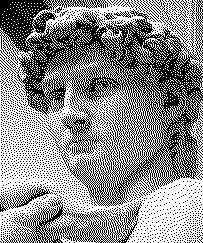
\includegraphics[width=0.25\textwidth]{figures/3c1.jpg}
    \caption
	{
خروجی الگوریتم \lr{Floyd-Steinberg}
	}
    \label{fig:fig1}
\end{figure}
\begin{figure}[H]
    \centering
    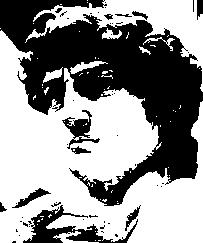
\includegraphics[width=0.25\textwidth]{figures/3c2.jpg}
    \caption
	{
خروجی الگوریتم حریصانه
	}
    \label{fig:fig1}
\end{figure}




%%%%%%%%%%%%%%%%%%%%%%%%%%%%%%%%%%%


%\begin{latin}
%\lstinputlisting{sources/p1.m}
%\end{latin}



%%%%%%%%%%%%%%%%%%%%%%%%%%%%%%%%%%%
%%%%%%%%%%%%%%%%%%%%%%%%%%%%%%%%%%%
%%%%%%%%%%%%%%%%%%%%%%%%%%%%%%%%%%%

%------------------------------------------------------------------------------------------


\section*{منابع}
\renewcommand{\section}[2]{}%
\begin{thebibliography}{99} % assumes less than 100 references
%چنانچه مرجع فارسی نیز داشته باشید باید دستور فوق را فعال کنید و مراجع فارسی خود را بعد از این دستور وارد کنید


\begin{LTRitems}

\resetlatinfont

\bibitem{b1}
\end{LTRitems}

\end{thebibliography}


\end{document}
